\documentclass[12pt]{article}
\usepackage[a4paper,margin=2.5cm]{geometry}
\usepackage{amsmath, amsfonts, amssymb, amsthm}
\usepackage{physics}
\usepackage{mathtools}
\usepackage{tikz}
\usetikzlibrary{angles,quotes}
\title{Entregables Distancias Topología}
\author{Juan Rodríguez}
\date{}
\begin{document}
\maketitle

\section*{Ejercicio 1}
Determinar cuáles de las siguientes funciones son distancias en $\mathbb{R}$.

\begin{enumerate}
\item $d(x,y) = |x - y|$. \\
Es distancia: cumple todos los axiomas de una métrica (distancia euclidiana). \\

Propiedad Reflexiva:
Si $x=y$, entonces $d(x,y) = 0$ \\
$d(x,x) = | x - x | = | 0 | = 0$ \\
Si $d(x,y) = 0$, entonces $x=y$ \\
$d(x,y) = |x - y| = 0 \rightarrow x - y = 0 \rightarrow x = y$ \\

Propiedad Simétrica: $d(x,y) = d(y,x)$ \\
$d(x,y) = | x - y | = | - (y - x) | = |y - x| = d(y,x)$ \\

Desigualdad Triangular: $d(x,z) \leq d(x,y) + d(y,z)$ \\
$d(x,z) = | x - z| \leq | x - y| + | y - z|$ \\
$a = x - y$ \quad $b = y - z$ \\
$|a + b| \leq |a| + |b|$

\item $d(x,y) = |x^2 - y^2|$. \\
No es distancia. Incumple la propiedad reflexiva \\
$d(1,-1)=0$ y $1\neq -1$. 

\item $d(x,y) = |x - 2y|$. \\
No es distancia. Incumple la propiedad reflexiva \\
$d(1,1) = 1 \neq 0$

\item $d(x,y) = (x - y)^2$. \\
No es distancia. Incumple la desigualdad triangular \\
$d(0,2) = 4 \not\leq 1 + 1 = d(0,1) + d(1,2)$

\item $d(x,y) = \sin^2(x - y)$. \\
No es distancia. Incumple la propiedad reflexiva \\
$d(x,y)=0 \rightarrow x - y = k\pi$, no solo cuando $x=y$.

\item $d(x,y) = \arctan|x - y|$. \\
Es distancia: cumple todos los axiomas de una métrica (distancia euclidiana). \\

Propiedad Reflexiva: \\
Si $x=y$, entonces $d(x,y) = 0$ \\
$d(x,x) = \arctan|x-x| = \arctan|0| = 0$ \\
Si $d(x,y) = 0$, entonces $x=y$ \\
$d(x,y) = \arctan|x-y| = 0 \rightarrow x - y = 0 \rightarrow x = y$ \\

Propiedad Simétrica: $d(x,y) = d(y,x)$ \\
$d(x,y) = \arctan| x - y | = \arctan| - (y - x) | = \arctan|y - x| = d(y,x)$ \\

Desigualdad Triangular: $d(x,z) \leq d(x,y) + d(y,z)$ \\
$d(x,z) = \arctan| x - z| \leq \arctan| x - y| + \arctan| y - z|$ \\
Tomamos tangente a ambos lados de la igualdad (Podemos hacerlo porque es una función monotona creciente, por lo que se cumple que $f(a) < f(b)$ si $a < b$) \\
$\tan(\arctan| x - z|) \leq \tan(\arctan| x - y| + \arctan| y - z|)$ \\

$\tan(a + b) = \frac{\tan(a)+\tan(b)}{1-\tan(a)\cdot\tan(b)}$ \\ 

$|x-z| \leq \frac{| x - y| + | y - z|}{1 - | x - y| \cdot | y - z|}$ \\
$|x-z| \leq | x - y| + | y - z| \leq \frac{| x - y| + | y - z|}{1 - | x - y| \cdot | y - z|}$

\end{enumerate}

\section*{Ejercicio 2}

Sea $d(A,B) = |A \cup B| - |A \cap B|$ para $A,B$ subconjuntos finitos de un conjunto universo $U$.

Propiedad Reflexiva: \\
Si $A=B$, entonces 
\[
d(A,A) = |A \cup A| - |A \cap A| = |A| - |A| = 0.
\]
Si $d(A,B)=0$, entonces $|A \cup B| = |A \cap B|$.  
Esto sólo puede ocurrir si $A=B$.  
Por tanto, $d(A,B)=0 \iff A=B$. \\

Propiedad Simétrica
\[
d(A,B) = |A \cup B| - |A \cap B| = |B \cup A| - |B \cap A| = d(B,A).
\]
Luego $d(A,B)$ es simétrica. \\

Desigualdad Triangular: \\
Queremos probar que
\[
d(A,B) \le d(A,C) + d(C,B).
\]

Empecemos escribiendo:
\[
d(A,B) = |A \cup B| - |A \cap B|.
\]

Por la fórmula de inclusión–exclusión:
\[
|A \cup B| = |A| + |B| - |A \cap B|,
\]
entonces
\[
d(A,B) = |A| + |B| - 2|A \cap B|.
\]

De modo análogo:
\[
d(A,C) = |A| + |C| - 2|A \cap C|, \qquad
d(B,C) = |B| + |C| - 2|B \cap C|.
\]

Sumando las dos últimas:
\[
d(A,C) + d(B,C) = |A| + |B| + 2|C| - 2|A \cap C| - 2|B \cap C|.
\]

La desigualdad triangular
\[
d(A,B) \le d(A,C) + d(B,C)
\]
es equivalente a
\[
|A| + |B| - 2|A \cap B| \le |A| + |B| + 2|C| - 2|A \cap C| - 2|B \cap C|.
\]

\[
-2|A \cap B| \le 2|C| - 2|A \cap C| - 2|B \cap C|.
\]

\[
-|A \cap B| \le |C| - |A \cap C| - |B \cap C|.
\]

\[
|A \cap C| + |B \cap C| - |A \cap B| \le |C|.
\]

\paragraph{Interpretación.}
El término de la izquierda representa los elementos de $C$ en común con $A$ y con $B$, restando los que se cuentan dos veces.  
Esa cantidad siempre es menor o igual que el número de elementos de $C$.  
Por tanto, la desigualdad se cumple y la desigualdad triangular queda demostrada.

\subsection*{Conclusión}
\[
\boxed{
d(A,B)=|A \cup B| - |A \cap B| \text{ es una métrica en la familia de subconjuntos finitos de } U.
}
\]

\section*{Ejercicio 3}
Determinar cuáles de las siguientes funciones son distancias en $\mathbb{R}^2$:
\[
\begin{aligned}
\text{a)}\;& d_2((x_1,y_1),(x_2,y_2))=\sqrt{(x_1-x_2)^2+(y_1-y_2)^2},\\
\text{b)}\;& d_\times((x_1,y_1),(x_2,y_2))=|x_1-x_2|\cdot|y_1-y_2|,\\
\text{c)}\;& d_1((x_1,y_1),(x_2,y_2))=|x_1-x_2|+|y_1-y_2|,\\
\text{d)}\;& d_{\min}((x_1,y_1),(x_2,y_2))=\min\{|x_1-x_2|,|y_1-y_2|\},\\
\text{e)}\;& d_\infty((x_1,y_1),(x_2,y_2))=\max\{|x_1-x_2|,|y_1-y_2|\}.
\end{aligned}
\]

Sean $p=(x_1,y_1)$, $q=(x_2,y_2)$, $r=(x_3,y_3)$.

\subsection*{a) Euclidiana $d_2$}
Si $p=q$, entonces $d(p,q)=0$ 

$d(p,p) = \sqrt{(0 + 0)} = 0$ \\

Si $d(p,q) = 0$, entonces $p=q$
$d(p,q)= 0 \rightarrow + (x_1-x_2)^2+(y_1-y_2)^2 = 0 \rightarrow $

$\rightarrow x_1 - x_2 = 0 \quad \text{y también que} \quad y_1 - y_2 = 0$

Por lo tanto $p=q$

\emph{Simetría:} $d_2(p,q)=d_2(q,p)$. \\

$d(p,q)=\sqrt{(x_1-x_2)^2+(y_1-y_2)^2} = \sqrt{(-(x_2-x_1))^2+(-(y_2-y_1))^2} = $ \\

$ = \sqrt{((x_2-x_1))^2+((y_2-y_1))^2} = d(q,p)$ \\

\emph{Desigualdad triangular:} Escribimos $u=q-p$, $v=r-q$ y $u+v=r-p$. Entonces
\[
d_2(p,r)=\|u+v\|
=\sqrt{(u_1+v_1)^2+(u_2+v_2)^2}
\le \|u\|+\|v\|,
\]
donde la última desigualdad es la de Minkowski. Por tanto, $d_2$ es distancia.

\subsection*{b) Producto $d_\times$}
No cumple la propiedad reflexiva: si $p\neq q$ pero comparten una coordenada, por ejemplo $p=(0,0)$, $q=(0,1)$, entonces
\[
d_\times(p,q)=|0-0|\cdot|0-1|=0\quad\text{con }p\neq q.
\]
No es distancia.

\subsection*{c) Manhattan $d_1$}
Propiedad Reflexiva:\\
Si $p=q$, entonces $d(p,q)=0$\\
$d(p,p) = 0 + 0 = 0$\\

Si $d(p,q)=0$ entonces $p=q$  \\
$d(p,q)=0 \rightarrow |x_1-x_2| = 0 \quad \text{y también que } \quad |y_1-y_2| = 0$

$\rightarrow p = q$ \\

\emph{Simetría:} $d_1(p,q)=d_1(q,p)$.

\emph{Desigualdad triangular:} usando la triangular en $\mathbb{R}$ para cada coordenada,
\[
|x_1-x_3|\le |x_1-x_2|+|x_2-x_3|,
\qquad
|y_1-y_3|\le |y_1-y_2|+|y_2-y_3|.
\]
Sumando,
\[
d_1(p,r)=|x_1-x_3|+|y_1-y_3|
\le (|x_1-x_2|+|x_2-x_3|)+(|y_1-y_2|+|y_2-y_3|)
= d_1(p,q)+d_1(q,r).
\]
Luego $d_1$ es distancia.

\subsection*{d) Mínimo $d_{\min}$}
Incumple la propiedad reflexiva: si $p\neq q$ y comparten alguna coordenada,
por ejemplo $p=(0,0)$, $q=(0,1)$,
\[
d_{\min}(p,q)=\min\{|0-0|,|0-1|\}=0\quad\text{con }p\neq q.
\]
No es métrica.

\subsection*{e) Máximo $d_\infty$}
Propiedad Reflexiva:
$d_\infty(p,q)=0\iff p=q$.

\emph{Simetría:} inmediata por el valor absoluto.

\emph{Desigualdad triangular:} con $u=q-p$, $v=r-q$ y $u+v=r-p$:
\[
\begin{aligned}
d_\infty(p,r)
&=\max\{|u_1+v_1|,|u_2+v_2|\}
\le \max\{|u_1|+|v_1|,\;|u_2|+|v_2|\}\\
&\le \max\{|u_1|,|u_2|\}+\max\{|v_1|,|v_2|\}
= d_\infty(p,q)+d_\infty(q,r).
\end{aligned}
\]
Por tanto, $d_\infty$ es métrica.


\section*{Ejercicio 4}
Sea $X=[0,1)$ y definamos, para $x,y\in X$,
\[
d(x,y)\;=\;\min\{|x-y|,\;1-|x-y|\}.
\]
Probar que $d$ es una distancia en $X$.

\subsection*{1)Reflexiva y simetría}
\begin{itemize}
\item \textbf{Reflexiva:} $d(x,y)=0\iff \min\{|x-y|,1-|x-y|\}=0\iff |x-y|=0 \iff x=y$ (como $|x-y|<1$ para $x,y\in[0,1)$).
\item \textbf{Simetría:} $d(x,y)=\min\{|x-y|,1-|x-y|\}=\min\{|y-x|,1-|y-x|\}=d(y,x)$.
\end{itemize}

\subsection*{2) Desigualdad triangular}
La idea es ver $X=[0,1)$ como el cociente $\mathbb{R}/\mathbb{Z}$ (la circunferencia), y expresar $d$ como un ínfimo de distancias euclidianas en $\mathbb{R}$. Para $x,y\in[0,1)$ definimos
\[
\tilde d(x,y)\;:=\;\inf_{k\in\mathbb{Z}}\,|x-y-k|.
\]
Observemos que, como $|x-y|\in[0,1)$, se tiene
\[
\tilde d(x,y)=\min\{|x-y|,\;1-|x-y|\}=d(x,y).
\]
Por tanto, basta probar la desigualdad triangular para $\tilde d$:
\[
\tilde d(x,z)\;\le\;\tilde d(x,y)+\tilde d(y,z)\qquad(\forall\,x,y,z\in[0,1)).
\]

Sea $m,n\in\mathbb{Z}$ arbitrarios. Usando la triangular en $\mathbb{R}$,
\[
|x-z-(m+n)|
= |(x-y-m)+(y-z-n)|
\le |x-y-m| + |y-z-n|.
\]
Tomando ínfimos (primero en $m,n$ y notando que $m+n$ recorre todo $\mathbb{Z}$), obtenemos
\[
\inf_{k\in\mathbb{Z}}|x-z-k|
\;\le\;
\inf_{m,n\in\mathbb{Z}}\big(|x-y-m|+|y-z-n|\big)
\;\le\;
\inf_{m\in\mathbb{Z}}|x-y-m|+\inf_{n\in\mathbb{Z}}|y-z-n|.
\]
Esto es, \(\tilde d(x,z)\le \tilde d(x,y)+\tilde d(y,z)\). Como $\tilde d=d$, la desigualdad triangular queda probada para $d$.

\subsection*{Conclusión}
Las tres propiedades (no negatividad y separación, simetría y desigualdad triangular) se cumplen. Luego
\[
\boxed{\,d(x,y)=\min\{|x-y|,\,1-|x-y|\}\ \text{define una métrica en }[0,1).\,}
\]

\paragraph{Observación.}
Esta es la \emph{distancia geodésica} en la circunferencia $S^1$ al identificar $0\sim 1$. 

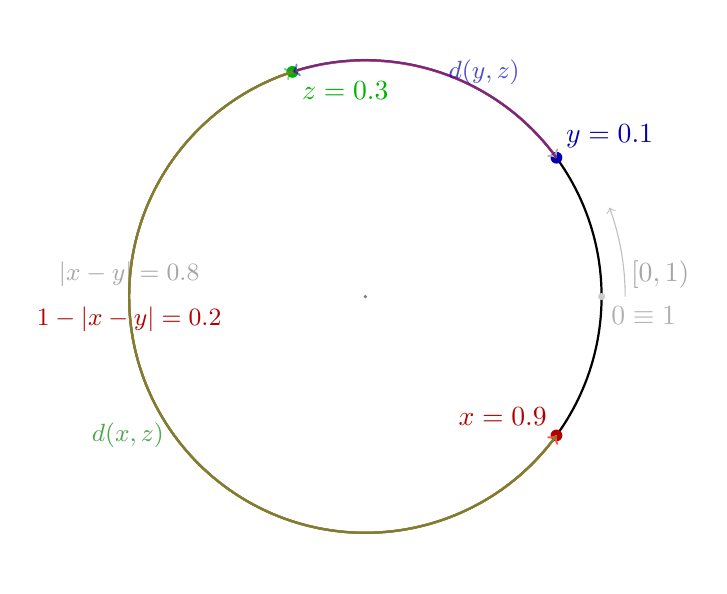
\begin{tikzpicture}[scale=3]
  % Círculo unidad (representa [0,1) con 0 y 1 identificados)
  \draw[thick] (0,0) circle (1);

  % Etiquetas para 0=1
  \draw[->,gray!50] (1.1,0) arc (0:20:1.1) node[midway,below right,gray!70] {$[0,1)$};
  \fill[gray!40] (1,0) circle (0.015) node[below right,gray!60] {$0\equiv 1$};

  % Puntos x=0.9, y=0.1, z=0.3
  \coordinate (x) at ({cos(360*0.9)},{sin(360*0.9)});
  \coordinate (y) at ({cos(360*0.1)},{sin(360*0.1)});
  \coordinate (z) at ({cos(360*0.3)},{sin(360*0.3)});

  \fill[red!70!black] (x) circle (0.025) node[above left] {$x=0.9$};
  \fill[blue!70!black] (y) circle (0.025) node[above right] {$y=0.1$};
  \fill[green!70!black] (z) circle (0.025) node[below right] {$z=0.3$};

  % Arco directo (largo)
  \draw[thick,gray!60,->] (x) arc (324:36:1)
    node[midway,above,gray!70] {\small $|x-y|=0.8$};

  % Arco más corto (usado por la métrica)
  \draw[thick,red!70,->] (y) arc (36:324:1)
    node[midway,below,red!70!black] {\small $1-|x-y|=0.2$};

  % Arcos de x-z y y-z (para la triangular)
  \draw[thick,green!70!black,->,opacity=0.5] (x) arc (324:108:1)
    node[midway,left,green!50!black,opacity=0.7] {\small $d(x,z)$};
  \draw[thick,blue!70!black,->,opacity=0.5] (y) arc (36:108:1)
    node[midway,right,blue!70!black,opacity=0.7] {\small $d(y,z)$};

  % Centro del círculo
  \fill[black!50] (0,0) circle (0.008);
\end{tikzpicture}

\section*{Ejercicio 5}
Sea $X$ un conjunto finito. Supongamos que $d:X\times X\to\{0,1\}$ es una distancia.
Probar que necesariamente $d$ coincide con la \emph{distancia discreta}
\[
\delta(x,y):=\begin{cases}
0,& x=y,\\[2pt]
1,& x\neq y.
\end{cases}
\]

Sea ahora $d:X\times X\to\{0,1\}$ una \emph{distancia} cualquiera.
\begin{itemize}
\item Por la propiedad reflexiva, $d(x,x)=0$ para todo $x\in X$.
\item Si $x\neq y$, entonces por reflexiva \emph{no} puede ocurrir $d(x,y)=0$; como el codominio es $\{0,1\}$, necesariamente $d(x,y)=1$.
\end{itemize}
Concluimos que, para todos $x,y\in X$, $d(x,y)=\delta(x,y)$. Es decir, \(
d=\delta
\).

\subsection*{Conclusión}
La única distancia en $X$ que toma valores exclusivamente en $\{0,1\}$ es la métrica discreta:
\[
\boxed{\ d(x,y)=0 \ \text{si } x=y,\quad d(x,y)=1 \ \text{si } x\neq y.\ }
\]

\section*{Ejercicio 6}
En $\mathbb{R}^2$, para $v=(x,y)$, demostrar
\[
\|v\|_2 \;\le\; \|v\|_1 \;\le\; \sqrt{2}\,\|v\|_2,
\qquad
\text{donde }\ \|v\|_1=|x|+|y|,\ \ \|v\|_2=\sqrt{x^2+y^2}.
\]

La cota derecha es equivalente a acotar la raz\'on
\[
R(x,y):=\frac{\|v\|_1}{\|v\|_2}=\frac{|x|+|y|}{\sqrt{x^2+y^2}}.
\]
Por simetr\'ia basta suponer $x\ge 0$ y $y\ge 0$ (los valores absolutos eliminan signos) y parametrizar $y=kx$ con $k\ge 0$ y $x>0$:
\[
R(x,y)=\frac{x+kx}{\sqrt{x^2+k^2x^2}}
=\frac{1+k}{\sqrt{1+k^2}}=:f(k).
\]
Buscamos $\max_{k\ge 0} f(k)$. Derivando,
\[
f(k)=\frac{1+k}{(1+k^2)^{1/2}},\qquad
f'(k)=\frac{(1+k^2)^{1/2}-(1+k)\,\dfrac{k}{(1+k^2)^{1/2}}}{1+k^2}
=\frac{1-k}{(1+k^2)^{3/2}}.
\]
Así, $f'(k)=0 \iff k=1$, con $f'(k)>0$ si $k<1$ y $f'(k)<0$ si $k>1$. Por tanto $k=1$ es m\'aximo global:
\[
\max_{k\ge 0} f(k) = f(1)=\frac{1+1}{\sqrt{1+1}}=\frac{2}{\sqrt{2}}=\sqrt{2}.
\]
Concluimos que para todo $(x,y)\ne(0,0)$,
\[
\frac{\|v\|_1}{\|v\|_2}\le \sqrt{2}
\quad\Longrightarrow\quad
\boxed{\ \|v\|_1 \le \sqrt{2}\,\|v\|_2\ }.
\]

Para la cota izquierda usamos que $(|x|+|y|)^2=x^2+y^2+2|xy|\ge x^2+y^2$, luego
\[
\boxed{\ \|v\|_2=\sqrt{x^2+y^2}\ \le\ |x|+|y|=\|v\|_1\ }.
\]

\subsection*{Conclusi\'on (equivalencia de m\'etricas)}
De las dos desigualdades obtenemos
\[
\boxed{\ \|v\|_2 \;\le\; \|v\|_1 \;\le\; \sqrt{2}\,\|v\|_2\ },
\]
así $d_1$ y $d_2$ son \emph{equivalentes} (inducen la misma topología).

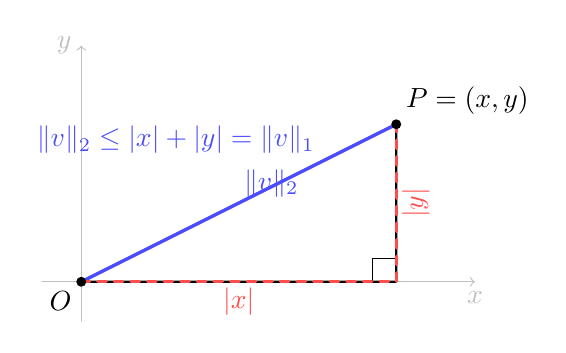
\begin{tikzpicture}[scale=1.0, line cap=round,line join=round]
  % Puntos
  \coordinate (O) at (0,0);
  \coordinate (X) at (4,0);
  \coordinate (Y) at (4,2);

  % Ejes (opcionales)
  \draw[->,gray!50] (-0.5,0) -- (5,0) node[below] {$x$};
  \draw[->,gray!50] (0,-0.5) -- (0,3) node[left] {$y$};

  % Triángulo rectángulo
  \draw[thick] (O) -- (X) -- (Y) -- cycle;

  % Marca de ángulo recto
  \draw (4,0) ++(-0.3,0) -- ++(0,0.3) -- ++(0.3,0);

  % Hipotenusa (Euclidiana)
  \draw[very thick,blue!70] (O) -- (Y) node[midway, above right=-2pt] {$\|v\|_2$};

  % Camino en L (Manhattan)
  \draw[very thick,red!70,dashed] (O) -- (X) -- (Y);
  \node[red!70] at (2,-0.25) {$|x|$};
  \node[red!70,rotate=90] at (4.25,1) {$|y|$};

  % Etiquetas
  \fill (O) circle (1.8pt) node[below left] {$O$};
  \fill (Y) circle (1.8pt) node[above right] {$P=(x,y)$};

  % Comentario
  \node[blue!70] at (1.2,1.8) {$\|v\|_2 \le |x|+|y|=\|v\|_1$};
\end{tikzpicture}

\section*{Ejercicio 7}
Sean $A,B,C\in\mathbb{R}^2$.

\subsection*{(a) Métrica taxicab continua en $\mathbb{R}^2$}
Definimos $d_1(P,Q)=|x_P-x_Q|+|y_P-y_Q|$. Probar que existe $O\in\mathbb{R}^2$
tal que $d_1(O,A)=d_1(O,B)=d_1(O,C)$.

\paragraph{Idea.}
El lugar geométrico de los puntos equidistantes a dos puntos $P,Q$:
\[
\mathcal{B}(P,Q):=\{X:\ d_1(X,P)=d_1(X,Q)\}
\]
es una línea poligonal no vacía formada por tramos con pendiente $\pm1$ (la “bisectriz $\ell^1$”).
Bastará ver que $\mathcal{B}(A,B)$ y $\mathcal{B}(A,C)$ \textit{siempre} se cortan.

\paragraph{Prueba (signos a lo largo de rectas).}
Sea, para $X=(x,y)$,
\[
F_{AB}(X):=d_1(X,A)-d_1(X,B).
\]
Tomemos la recta $\gamma(t)=(t,-t)$. Entonces $t\mapsto F_{AB}(\gamma(t))$ es continua y,
para $|t|$ grande, los valores absolutos se “despegan”, quedando
\[
F_{AB}(\gamma(t))=
|t-a_x|+|-t-a_y|-|t-b_x|-|-t-b_y|
=
\big(a_y-a_x\big)-\big(b_y-b_x\big)\quad\text{para }t\gg 1,
\]
mientras que, para $t\ll -1$,
\[
F_{AB}(\gamma(t))=
\big(a_x-a_y\big)-\big(b_x-b_y\big)
= -\Big[\big(a_y-a_x\big)-\big(b_y-b_x\big)\Big].
\]
Por el teorema del valor intermedio, existe $t_0$ tal que $F_{AB}(\gamma(t_0))=0$; es decir,
$\gamma(t_0)\in\mathcal{B}(A,B)$. Un razonamiento idéntico (por ejemplo sobre la recta
$\eta(s)=(s,s)$) muestra que $\mathcal{B}(A,C)$ también corta a alguna recta de pendiente $+1$.
Como $\mathcal{B}(A,B)$ tiene tramos de pendiente $+1$ y $-1$ (y lo mismo $\mathcal{B}(A,C)$),
y ambos son no acotados en el plano, necesariamente
\[
\mathcal{B}(A,B)\cap\mathcal{B}(A,C)\neq\varnothing.
\]
Cualquier punto $O$ en la intersección cumple $d_1(O,A)=d_1(O,B)=d_1(O,C)$.

\paragraph{Conclusión.}
En $(\mathbb{R}^2,\ell^1)$ siempre existe (aunque puede no ser único) un punto
$O$ equidistante a $A,B,C$.

\subsection*{(b) Métrica taxicab discreta en $\mathbb{Z}^2$}
Ahora $A,B,C\in\mathbb{Z}^2$ y buscamos $O\in\mathbb{Z}^2$ con
$d_1(O,A)=d_1(O,B)=d_1(O,C)$.

\paragraph{Afirmación.}
Tal $O$ existe \textbf{si y sólo si}
\[
a_x+a_y\equiv b_x+b_y\equiv c_x+c_y \pmod 2.
\]

\paragraph{Necesidad (condición de paridad).}
Sea $O=(u,v)\in\mathbb{Z}^2$. Como $|m|\equiv m\ (\mathrm{mod}\ 2)$ para $m\in\mathbb{Z}$,
\[
d_1(O,P)=|u-p_x|+|v-p_y|\equiv (u-p_x)+(v-p_y)=
(u+v)-(p_x+p_y)\pmod 2.
\]
Si $d_1(O,A)=d_1(O,B)$, entonces
\[
(u+v)-(a_x+a_y)\equiv (u+v)-(b_x+b_y)\pmod 2
\ \Rightarrow\ 
a_x+a_y\equiv b_x+b_y\ (\mathrm{mod}\ 2).
\]
Aplicando a los tres pares, todas las sumas deben tener la \emph{misma} paridad.

\paragraph{Suficiencia (construcción).}
Supongamos $a_x+a_y\equiv b_x+b_y\equiv c_x+c_y\ (\mathrm{mod}\ 2)$.
La bisectriz $\ell^1$ de dos puntos de \(\mathbb{Z}^2\) con la misma paridad
\emph{sí} contiene puntos de la retícula (sus tramos de pendiente $\pm1$
pasan por vértices de la cuadrícula), mientras que si las paridades difieren,
la bisectriz “queda entre” nodos de la retícula.

Sea $L_{AB}:=\mathcal{B}(A,B)\cap\mathbb{Z}^2$ y $L_{AC}:=\mathcal{B}(A,C)\cap\mathbb{Z}^2$.
Bajo la hipótesis de paridad común, ambas son no vacías y, como en la parte continua,
tienen tramos infinitos en direcciones de pendiente $\pm1$. Dos tales conjuntos
infinito–rectilíneos en direcciones cruzadas \emph{siempre} se intersecan en algún
nodo de la retícula; sea $O\in L_{AB}\cap L_{AC}$. Entonces
\[
d_1(O,A)=d_1(O,B)=d_1(O,C),
\]
con $O\in\mathbb{Z}^2$.

\paragraph{Conclusión.}
En la retícula $(\mathbb{Z}^2,\ell^1)$ existe $O\in\mathbb{Z}^2$ equidistante a $A,B,C$
\emph{ssi} $a_x+a_y$, $b_x+b_y$ y $c_x+c_y$ tienen la misma paridad.

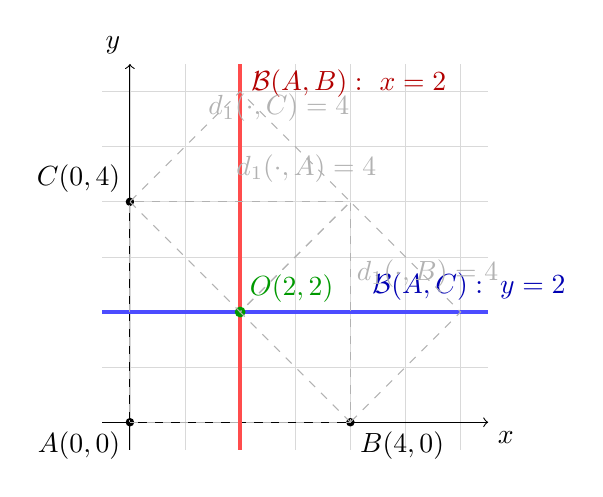
\begin{tikzpicture}[scale=0.7]
  % Cuadrícula para ver la retícula Z^2
  \draw[help lines,step=1,gray!30] (-0.5,-0.5) grid (6.5,6.5);

  % Ejes
  \draw[->] (-0.5,0) -- (6.5,0) node[below right] {$x$};
  \draw[->] (0,-0.5) -- (0,6.5) node[above left] {$y$};

  % Puntos A, B, C
  \fill[black] (0,0) circle (2.2pt) node[below left] {$A(0,0)$};
  \fill[black] (4,0) circle (2.2pt) node[below right] {$B(4,0)$};
  \fill[black] (0,4) circle (2.2pt) node[above left] {$C(0,4)$};

  % Bisectriz L1 de A y B: x = 2 (vertical)
  \draw[line width=1.4pt,red!70] (2,-0.5) -- (2,6.5)
     node[pos=0.95,right,red!70!black] {$\mathcal B(A,B):\ x=2$};

  % Bisectriz L1 de A y C: y = 2 (horizontal)
  \draw[line width=1.4pt,blue!70] (-0.5,2) -- (6.5,2)
     node[pos=0.95,above,blue!70!black] {$\mathcal B(A,C):\ y=2$};

  % Punto O de intersección
  \fill[green!60!black] (2,2) circle (2.8pt) node[above right] {$O(2,2)$};

  % (Opcional) Diamantes (círculos L1) de radio 4 que se encuentran en O
  \draw[gray!60,dashed] (0,0) -- ++(4,0) -- ++(0,4) -- ++(-4,0) -- cycle;
  \draw[gray!60,dashed] (4,0) -- ++(-2,2) -- ++(2,2) -- ++(2,-2) -- cycle;
  \draw[gray!60,dashed] (0,4) -- ++(2,-2) -- ++(2,2) -- ++(-2,2) -- cycle;
  \node[gray!60] at (3.2,4.6) {$d_1(\cdot,A)=4$};
  \node[gray!60] at (5.4,2.7) {$d_1(\cdot,B)=4$};
  \node[gray!60] at (2.7,5.7) {$d_1(\cdot,C)=4$};
\end{tikzpicture}

\subsection*{Ejercicio 8}
Calcular el valor análogo a $\pi$ en la métrica taxicab.

\medskip
En $\ell^1$, el círculo de radio $r$ es un rombo de perímetro $8r$ y diámetro $2r$, luego
\[
\pi_{\text{taxi}} = \frac{\text{perímetro}}{\text{diámetro}} = \frac{8r}{2r} = 4.
\]

\section*{Ejercicio 9}
Sea $f(x)=\sin(2x)$ y $g(x)=\cos x$ en $[0,\pi]$.
Queremos calcular
\[
d_1(f,g)=\int_0^\pi |f(x)-g(x)|\,dx,
\qquad
d_\infty(f,g)=\sup_{x\in[0,\pi]} |f(x)-g(x)|.
\]

\subsection*{Preparación}
\[
f(x)-g(x)=\sin(2x)-\cos x
= \underbrace{\cos x}_{(\*)}\,\underbrace{(2\sin x-1)}_{(\*\*)}.
\]
Los ceros relevantes (cambios de signo) son:
\[
\cos x=0 \iff x=\frac{\pi}{2}, \qquad
2\sin x-1=0 \iff \sin x=\tfrac12 \iff x=\frac{\pi}{6},\frac{5\pi}{6}.
\]
Con esto, el intervalo $[0,\pi]$ se parte en
\[
[0,\tfrac{\pi}{6}],\quad
(\tfrac{\pi}{6},\tfrac{\pi}{2}],\quad
(\tfrac{\pi}{2},\tfrac{5\pi}{6}),\quad
[\tfrac{5\pi}{6},\pi],
\]
en los que el signo de $\cos x(2\sin x-1)$ es, respectivamente,
\[
-,\ +,\ -,\ +.
\]

\subsection*{a) Distancia integral $d_1$}
Escribimos
\[
d_1(f,g)=\int_0^\pi \big|\cos x\,(2\sin x-1)\big|\,dx.
\]
Para quitar el valor absoluto, integramos por tramos invirtiendo el signo
donde el producto es negativo:
\[
\begin{aligned}
d_1(f,g)
&=\Big(
-\!\!\int_{0}^{\pi/6}
+\int_{\pi/6}^{\pi/2}
-\!\!\int_{\pi/2}^{5\pi/6}
+\int_{5\pi/6}^{\pi}
\Big)\big(\cos x\,(2\sin x-1)\big)\,dx\\[2mm]
&=\Big(
-\!\!\int_{0}^{\pi/6}
+\int_{\pi/6}^{\pi/2}
-\!\!\int_{\pi/2}^{5\pi/6}
+\int_{5\pi/6}^{\pi}
\Big)\big(\sin 2x-\cos x\big)\,dx.
\end{aligned}
\]
Tomamos una primitiva
\[
P(x)=\int (\sin 2x-\cos x)\,dx
=-\frac{1}{2}\cos 2x-\sin x.
\]
Evaluamos en los puntos de corte (valores exactos):
\[
\begin{array}{c|ccccc}
x & 0 & \frac{\pi}{6} & \frac{\pi}{2} & \frac{5\pi}{6} & \pi \\ \hline
\cos 2x & 1 & \frac{1}{2} & -1 & \frac{1}{2} & 1 \\
\sin x  & 0 & \frac{1}{2} & 1 & \frac{1}{2} & 0 \\
P(x)    & -\tfrac12 & -\tfrac34 & -\tfrac12 & -\tfrac34 & -\tfrac12
\end{array}
\]
Ahora, tramo a tramo (con el signo correspondiente):
\[
\begin{aligned}
I_1&=-\big(P(\tfrac{\pi}{6})-P(0)\big) = -\big(-\tfrac34+ \tfrac12\big)=\tfrac14,\\
I_2&= \ \big(P(\tfrac{\pi}{2})-P(\tfrac{\pi}{6})\big)= -\tfrac12-(-\tfrac34)=\tfrac14,\\
I_3&=-\big(P(\tfrac{5\pi}{6})-P(\tfrac{\pi}{2})\big)= -\big(-\tfrac34+ \tfrac12\big)=\tfrac14,\\
I_4&= \ \big(P(\pi)-P(\tfrac{5\pi}{6})\big)= -\tfrac12-(-\tfrac34)=\tfrac14.
\end{aligned}
\]
Sumando:
\[
d_1(f,g)=I_1+I_2+I_3+I_4=\tfrac14+\tfrac14+\tfrac14+\tfrac14=\boxed{1}.
\]

\subsection*{b) Distancia del supremo $d_\infty$}
Como $x\in[0,\pi]$,
\[
|\cos x|\le 1,\qquad \sin x\in[0,1]\ \Rightarrow\ 2\sin x-1\in[-1,1]\ \Rightarrow\ |2\sin x-1|\le 1.
\]
Por tanto,
\[
|f(x)-g(x)|=\big|\cos x\,(2\sin x-1)\big|\le 1\cdot 1=1.
\]
Este cota es alcanzable en $x=0$ y $x=\pi$:
\[
|f(0)-g(0)|=|\sin 0-\cos 0|=|0-1|=1,\qquad
|f(\pi)-g(\pi)|=|\sin 2\pi-\cos\pi|=|0-(-1)|=1.
\]
Luego
\[
d_\infty(f,g)=\sup_{x\in[0,\pi]} |f(x)-g(x)|=\boxed{1}.
\]

\end{document}